\begin{figure}
    \centering
    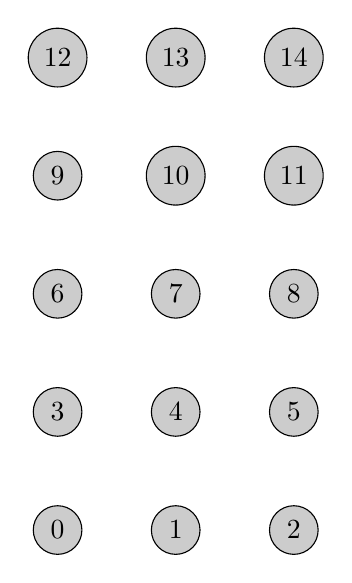
\begin{tikzpicture}[darkstyle/.style={circle,draw,fill=gray!40,minimum size=15}]
        \pgfmathsetmacro {\lx }{2}
        \pgfmathsetmacro {\ly }{4}
        \pgfmathtruncatemacro{\nnodes }{(1+\lx) * (1+\ly)}
        \pgfmathtruncatemacro{\nodes }{\nnodes-2}

        \foreach \x in {0,...,\lx}
        \foreach \y in {0,...,\ly}{
            \pgfmathtruncatemacro{\n}{\x + (1+\lx)*\y} 
            \node [darkstyle]  (\n) at (1.5*\x,1.5*\y) {\n};
        } 
        
%        \foreach \n in {0,...,\nodes}{
%            \pgfmathtruncatemacro{\m}{\n+1}
%            \draw (\n)--(\m);
%        }
    \end{tikzpicture}
    \caption{Finite size quantum well}
\end{figure}